\scanpage{69}
\diagram{\begin{tikzcd}[ampersand replacement=\&,column sep=large]
\&K(x)\arrow[r,very thick,"x\geq y"]\&K(y)\arrow[dr]\\
K(x')\arrow[ur]\arrow[rrr,no head]\&\&\&K(y')
\end{tikzcd}}
\[
x'\geq\underbrace{x\geq y}\geq y'
\]
\[
H(x,y)\longrightarrow H(x',y')
\]
\unsure{chaque fois qu'on se donne un chemin saturé} \unsure{joignant} $x$ à $x'$ et un \unsure{autre} joignant $y'$ à $y$.
\[
y'\rightsquigarrow\longleftrightarrow x\rightsquigarrow x'
\]
\unsure{Si} : \unsure{tout} \unsure{chemin|chaîne} \unsure{saturée|saturé} $s$ joignant $x$ à $y$, on associe $H_s=H(x,y)$, alors si $s\leq s'$, alors $H_s\longrightarrow H_{s'}$ ; \deleted{d'ailleurs $H_{\unsure{s'|s}}$ est \unsure{engendré} par les images des $H_{s'}$, \unsure{ou|où} $s'\leq s$, $s'$ \uline{\unsure{contigu}} à $s$}
\figure{\begin{tikzpicture}
\draw[line width=2pt] (0,1.4)--(1.2,1.4);\draw (.6,1.3)--(.6,1.55);\draw(0,1.2)--(.55,1.2);\fill(0,1.4)circle(2pt)(1.2,1.4)circle(2pt);
\draw (5,1.4)--(8,1.6);\fill (4.8,1.4)circle(1.5pt)(8,1.6)circle(2pt);
\draw (0,0)--(4,.03);\draw (0,-.12)--(0,.12) (.6,-.13)--(.6,.15);\fill (4,.03)circle(2pt);
\end{tikzpicture}}
\[
H_s\quad s\text{ de longueur }0\qquad
H_s\quad s\text{ de longueur }1
\]
\figure{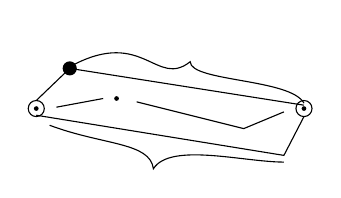
\begin{tikzpicture}[scale=.85]
\draw (0,0)circle(.12);\fill(0,0)circle(1pt)(.5,.6)circle(3pt);\draw (4,0)circle(.12);\fill(4,0)circle(1pt);
\draw (0,.12)--(.5,.6)--(4,.05) (0,-.1)--(3.7,-.7)--(4,-.12);
\draw (.3,.02)--(1,.15);\fill(1.2,.15)circle(1pt);\draw(1.5,.1)--(3.1,-.3)--(3.7,-.05);
\draw (.55,.65)..controls(1.6,1.2)and(1.8,.3)..(2.3,.7)..controls(2.3,.4)and(3.8,.45)..(4,.08);
\draw (.2,-.25)..controls(1,-.55)and(1.7,-.5)..(1.75,-.9)..controls(2,-.5)and(3.1,-.8)..(3.7,-.8);
\end{tikzpicture}}
\figure{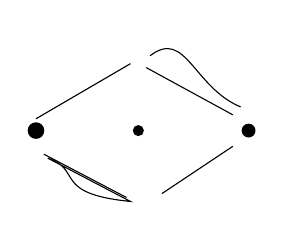
\begin{tikzpicture}
\fill(0,0)circle(3pt)(1.3,0)circle(2pt)(2.7,0)circle(2.5pt);
\draw (0,.15)--(1.2,.85) (1.4,.8)--(2.5,.2) (2.5,-.2)--(1.6,-.8) (.1,-.3)--(1.15,-.85);
\draw (1.45,.95)..controls(1.9,1.3)and(2,.55)..(2.6,.3);
\draw (.15,-.35)..controls(.6,-.5)and(.2,-.8)..(1.2,-.9)--(.15,-.35);
\end{tikzpicture}}
\diagram{\begin{tikzcd}[ampersand replacement=\&]
\left(\displaystyle\coprod_{s\in C_2(x,y)}H_s\right)\left(\displaystyle\coprod_{t\in C_{\unsure{1|2}}(x,y)}H_t\right)\\
H_{s\in C_0(x,y)}\arrow[u]
\end{tikzcd}}
\[
K_n=\coprod H_s\qquad\prod_x H\left(x,\coprod y\right)
\]
\[
\prod_x\prod_{y\,\text{\unsure{loc}}}H(x,y)
\]
\diagram{\begin{tikzcd}[ampersand replacement=\&,column sep=tiny]
{}\arrow[r,very thick]\arrow[rrr,dashed,bend right]\&{}\arrow[r]\&{}\arrow[r]\&{}\arrow[r]\&{}\arrow[r]\&{}\arrow[r]\&{}
\end{tikzcd}}
$I$ \unsure{ensemble ordonné} ``discret'' \unsure{au sens large}

$\widetilde I$ \unsure{catégorie des flèches composées}

$K$ \deleted{$\unsure{K}$} \unsure{foncteur} de $\widetilde I$ dans $C$
% archive sheet number: 68
